\documentclass[a4paper,12pt]{report}
\usepackage{cmap} % Поиск PDF
\usepackage[T2A]{fontenc}  % Кодировка
\usepackage[utf8]{inputenc}  % Кодировка исходного текста 
\usepackage[english]{babel}  % Кодировка исходного текста 
\usepackage{fontspec}
\usepackage{xcolor}
\usepackage{hyperref}
\definecolor{linkcolor}{HTML}{2d7ac7} % цвет ссылок
\definecolor{urlcolor}{HTML}{2d7ac7} % цвет гиперссылок
\usepackage{graphicx}
\graphicspath{ {./images/} }

\newcommand{\contractAddress}{0x37d29cb7d543300063a50d85389d409c01da7945}

\hypersetup{pdfstartview=FitH,  linkcolor=linkcolor,urlcolor=urlcolor, colorlinks=true}

\setmainfont{Ubuntu}
\providecommand{\versionnumber}{1.1}

% Title Page
\title{
\includegraphics[width=14cm]{logo}\\[2cm]Portal Energy Infrastructure \\\normalsize v\versionnumber}
\author{Ivantsov M. Movchan P. Prusov M. Butakov S. Patrikeev B.}

\date{\today}


\begin{document}%
\maketitle
\tableofcontents
\clearpage


\chapter{Introductuion}

Portal Energy was founded on the fusion of technologies in the field of electronics and Blockchain. Since 2016  we have been working on creating inexpensive and universal charging stations  for electric vehicles, understanding   their importance  for our country and humanity in the near future. At that time, we clearly mapped out our way  as a manufacturing  company and gained experience from each order.

We have a clear understanding that infrastructure is not just a stand-alone station that transmits electricity to electric vehicles, but an entire ecosystem that can significantly decrease the  population's  expenses   on energy sources, optimize the operation of the power grid  and contribute to the development of new industries and markets, such as renewable energy, energy storage  and smart cities. That's  why  we recruit specialists from these fields  in  our team.

We will use various technical terms in the text below. Their brief explanation is given in the Glossary. If you are familiar with them, then  you can go straight to section \ref{chapter3}.


\chapter{Glossary}

\section{Smart contract}
Smart contracts are similar to classic contracts, apart from the fact that a lot of people can act as the  third party.They check the contract for its execution and the result of this must match for all participants, only then it will be considered as a correct one.

In contract, we can specify any conditions that need to be fulfilled. Due to the fact that it is performed by many participants, we can not afford to execute very complex contracts, because they will require a lot of computing power. The calculation fee is charged in ETH currency  (Ethereum network). After the contract is executed, its state is saved in blockchain, and it is impossible to delete this information.


\section{Blockchain}
A continuous sequential chain of blocks containing information,  built according to certain rules. In simple words, it is a chain of blocks, each of which has a timestamp, a link to the previous block, and is stored on different computers.

\section{Cryptocurrency}
An encrypted unregulated digital asset that is used as a currency substitute in exchange operations. Cryptocurrency has no physical form, it exists only in electronic form as a data.
The unit of such a currency is "coin ". “Coin”  is fraud-proof, since it is encrypted information that cannot be copied.


\section{Ethereum}
A platform for creating decentralized online services on blockchain basis (decentralized applications)  and running on smart contract database. Implemented as a single decentralized VM.(Virtual Machine)

\section{Ether}
The exchange unit of Ethereum is called ether. It can be divided into fractional parts. 1/1000 — finney, 1/106 —szabo, 1/1018 — wei. This currency can be used by both  regular wallet or a smart contract. The POE token has the same properties.

\section{Token}
A non-cryptocurrency accounting unit which is used  for the representation of digital balance in some assets, in other words, performing the function of a "substitute for securities" in digital world. Tokens are represented as a registry entry, distributed in the blockchain.

\section{ERC20 Token}
ERC (Ethereum Request for Comments) is an official protocol to make suggestions for improving the Ethereum network, it uses an unique offer id number. Technical specifications for tokens issued on the Ethereum blockchain were published in 2015. Tokens that meet these specifications are known as ERC-20 tokens and are actually Ethereum blockchain smart contracts. The ERC-20 standard defines a set of rules that must be followed so that  token could be accepted and able to interact with other tokens in the network. The tokens themselves are blockchain assets that can have value, and can also be sent and received like any other cryptocurrency.
The difference between ERC-20 tokens and other well-known cryptocurrencies, such as Bitcoin or Litecoin  is that they are linked to the Ethereum network, use the address format accepted within Ethereum  network and are sent using Ethereum transactions. Accordingly, transactions with  ERC-20 tokens can be tracked in “block” explorers..

\href{https://etherscan.io/address/\contractAddress}{Here} you can track the movement of all our tokens.


\section{Private Blockchain}
All networks, such as Bitcoin, Ethereum, and EOS, are public, because anyone can write data to  this network anonymously , which makes its bandwidth more limited.  You`re not always want to publish some confidential data in public network and if the transaction has a heavy smart contract with complex logic, then you can face with  too high commission. So basically,  we have a lot of restrictions. Therefore, private blockchain systems such as Substrate (Polkadot framework) Hyperledger Fabric, Hyperledger Sawtooth, Quorum and others are more suitable for business. Due to the fact that only authorized participants, that  we  know, can write to this network, we have scalable bandwidth and no transaction fees. The only expenses for  business is the infrastructure support, i.e. the server and specialists who support the system.


\section{Etherscan}
This is the service for viewing Ethereum network stats. The main function of Etherscan is tracking of ongoing transactions. You can use it to check the status of your operation.  To check addresses and get more information, please visit \href{https://etherscan.io/}{https://etherscan.io/}.


\chapter{Electric vehicles as a technology}
\label{chapter3}
We are confident that electric vehicles are the future of  car  industry. Why ? First of all, due to the fact that  electric motor is much more efficient than the  internal combustion engine (hereinafter ICE) (The efficiency of  electric motor is 95-98\% VS  38\% ICE). Which in itself translates into significant savings (based on 100 km, charging an electric vehicle is 5-6 times cheaper than gasoline one ). In addition, the electric drive is eco-friendly, which is extremely important for residents of mega-cities.  Generally, the  environmental issue is becoming more and more relevant.

And furthermore,  due to design differences, electric vehicles are much more maneuverable and safer than  gasoline cars. And finally, the potential of electric vehicle  is just beginning to unleash, while  the potential of ICE car has already reached its limit. For example, the autopilot system can only be fully implemented in  electric vehicle.
One may then logically ask,  if electric cars are better  according for most indicators, they are much cheaper to operate and charge and are eco-friendly - why they are not widely distributed in our country?

This brings us to our second question:


\chapter{Why  there is  no widespread  infrastructure development in Russia?}
This is a really good question. But to answer this clearly, let's  have a look at countries where electric transport is already widespread.

\section{Electric vehicles worldwide}
The best situation with electric vehicles now in China. Only in 2019, more than 1.2 million new cars were registered there, 3.8 million total. Also, at the beginning of 2019  more than 1 million charging stations were officially registered there.
The USA is in second place. 330,000 electric vehicles were officially registered there in 2019 and more than 1.5 million  total. Also more than 200 thousand charging stations were already  there for 2019.
In Europe, at the end of 2019, the number of electric vehicles approached 2 million units, with 550 thousand units sold and 50\% increase in sales at the beginning of 2020. Moreover, the future of electric transport in developed countries is really promising.
Just have a look at  EV producing growth charts. These indicators speak for themselves. Also, it should be noted that this statistic includes not only electric vehicles, but also plug-in hybrids, since the vast majority of them have quite capacious batteries and fully use the charging infrastructure. After 2023, the number of such hybrids will decrease in favor of electric vehicles.
Numbers in “triangles”  below indicate some important events that accelerate the change of vehicle fleet on the planet from ICE to electric power  or important checkpoints  of these changes.

\vspace*{1cm}
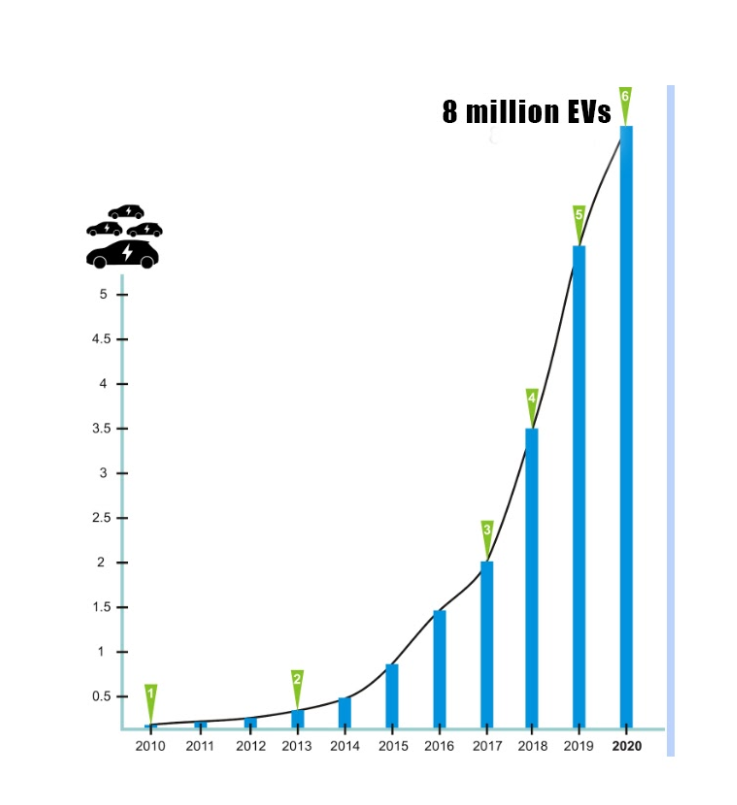
\includegraphics[width=12cm]{chart1en}
\vspace*{1cm}

\begin{enumerate}
	\item The  world first mass - produced electric vehicle  in modern history- Nissan Leaf
	\item Tesla Model S release
	\item Tesla Model 3 release
	\item Every 3rd vehicle  in Norway is electric one
	\item The number of charging stations in Europe has exceeded the number of gas stations
	\item More than 1 million Tesla cars sold
\end{enumerate}



\vspace*{1cm}
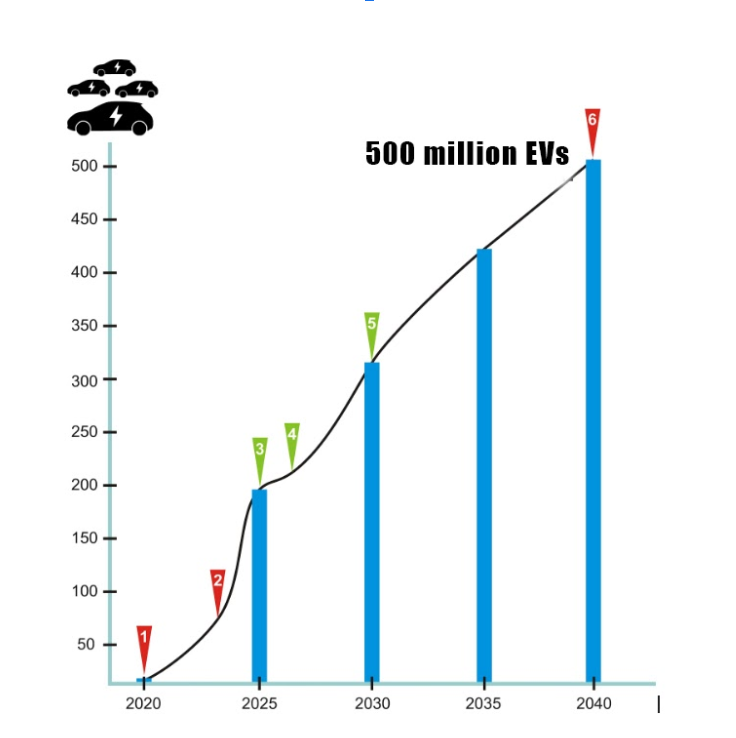
\includegraphics[width=12cm]{chart2en}
\vspace*{1cm}

\begin{enumerate}
	\item A car manufacturers such as BMW, Mercedes, Volvo, Audi, Volkswagen, Toyota  refused their  further development in the field of internal combustion engines
	\item the aligning  of  electric vehicles cost  with the ICE vehicles ( due to lowering the cost of batteries)
	\item the beginning of self-driving  and  commercial electric vehicles spreading
	\item Toyota and Volkswagen stop producing  ICE  vehicles
	\item Ban on the ICE cars using in the Netherlands, Sweden, Scotland, Denmark and Israel
	\item Total ban on the  ICE  cars in Europe
\end{enumerate}


What conclusions can we draw from the given data? Now we are at the dawn of the new  transport era. In all developed countries, the transition to electric vehicles is in full swing, and this is not just the imagination of some enthusiasts, but the specific intent of the biggest automotive giants.
However, a bright future will not come on its own.. We must build it!


\section{Electric vehicles in Russia}
Now, for instance, there are only  about \textbf{500}  charging stations in Russia. To understand  the future of electric cars, let's have a look at  the ICE vehicles from this perspective. Would you like to buy a car that could only be fueled in 500 locations throughout Russia? Which are not being maintained properly and  clear vision development  of which is not expected. Probably not,  which makes sense, because a  car is not bought for self-torture, but to level up personal freedom and comfort travelling. Therefore, an unavoidable condition for increasing the number of electric vehicles and their comfortable operation is the development of  charging infrastructure.


\chapter{The problem of EV charging infrastructure}
In addition to the  insufficient number of stations in our country, most of them are located in  strange and inconvenient places for car owners. They also don't have proper service and  appropriate information support. Basically, these stations are owned by state  companies  with all theirs consequences. Therefore, we are convinced that the development of electric transport in Russia should begin with the creation of an appropriate and convenient infrastructure.

This is precisely the goal that Portal Energy Team puts before itself.


\chapter{We are enthusiasts of this movement}
We want to unite other enthusiasts in Russia and around the world.
Now everyone is hoping that someone with Big money  will  start developing infrastructure, but it is already possible to do with  our \textbf{community}!

Additional incentives for us are design and urbanism. It is necessary to fill modern cities with a really inspiring technical objects and charging stations  are the best solution. We attach great importance to their design and structural features!
Our production is located in Saint-Petersburg. It includes metalworking shop, plastic molding shop and assembly area. All hardware is assembled and programmed separately.
We are convinced that a wide range of people should participate in the process of creating the charging infrastructure. This will provide the best quality, price of  charging stations and services, as well as contribute to rapid expansion of electric transport all over the world. A clear \textbf{investment program} has been developed for this purpose.
We design our charging stations based on advanced technical solutions and constantly analyze human interaction with this  infrastructure. Thanks to keen interest in our activities, a modern people  community begins to grow around Portal Energy. They  seriously cares about our future and  could affect it!


\chapter{Infrastructure development plan}

The first thing we have to do is to create a tool for effective interaction. Portal Energy is already such a tool.

The second one, we need a manufacturer that could satisfy the need in  future charging stations infrastructure and  take the responsibility  for  their maintenance. Portal Energy is already such a manufacturer.

Also an important factor in  development of electric transport infrastructure, is the understanding of its specifics. The behavior model of an electric car owner differs from the behavior model of  ICE vehicle owner. The location of gas stations  due to  technical restrictions  are always located in such places where you can physically build  and  service it properly. The owner  of ICE car is  necessarily depends on  gas station locations and this  is a  " pain”  which he has to contend with.

As regards the question of charging station, it can be located in  convenient  place  for the car owner,because the space requirements for installing charging stations are insignificant. And, therefore, when developing a map of station locations, it is necessary to rely primarily on the location of electric vehicles owners. And only in this case, charging car process  will no longer be an inevitable headache for the owner and  become a simple, clear and  stress free action. The owner could charge his  car not only during the travelling but when he minds his own business, since there will  be always  a charging station in every convenient place.

In big cities, the most reasonable places to start infrastructure development are shopping  malls and business centers, from which the  charging stations  chain will stretch to all  the areas.
Stations which are  located every 50-100 km between the cities  can completely solve the problem of charging  during a long trip.
This is how we see the logic of infrastructure development.

\begin{center}
	\textbf{Here are the main milestones in the development of our project for the next year}
\end{center}

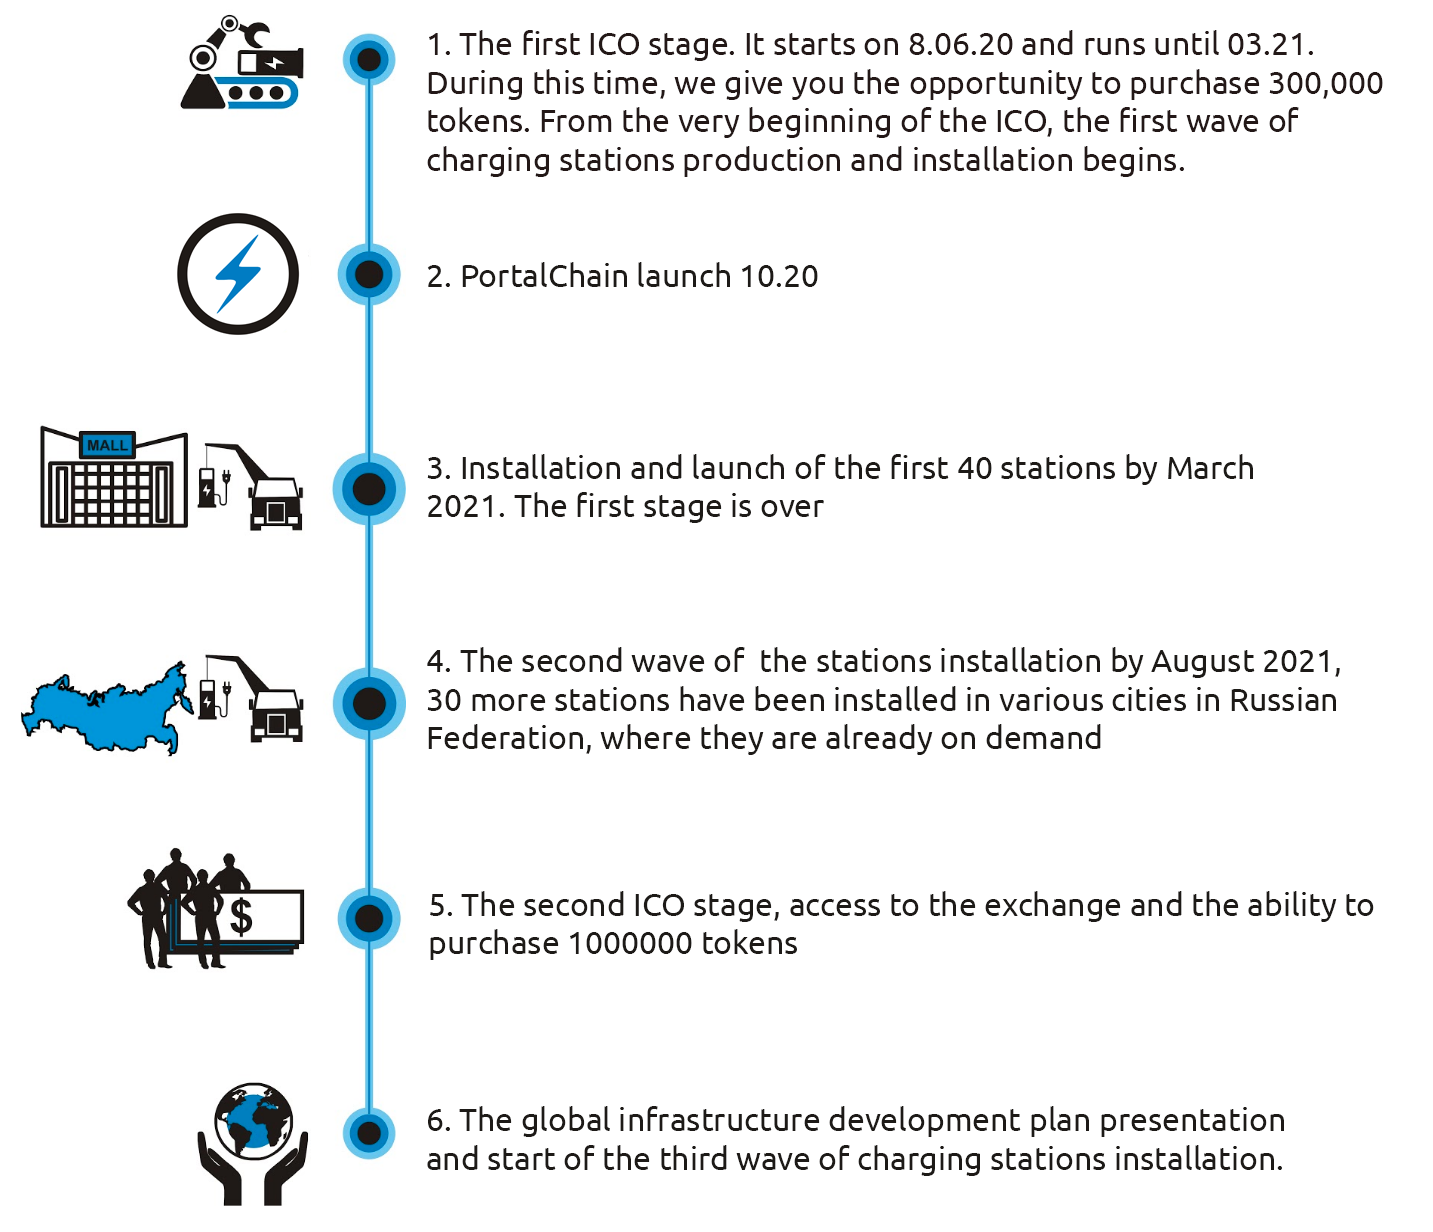
\includegraphics[width=13cm]{roadmapen}
\vspace*{1cm}

\chapter{Company structure}

Since such a task can only be solved under the conditions of absolute trust  of all the members, then we had to build such a confidence. In our opinion, the best foundation for establishing a  trusting relationship is a full transparency of all financial processes in the organization. And to provide  such transparency, we chose the \textbf{blockchain}.

The process  is rather simple. For example, the cost of one station is \$ 4,000. 5 people bought tokens and covered this sum.
We produce this station  (at the lowest possible price) , install  it  in the Parking lot of the shopping malls and connect it to the network. Then a revenue from the station will be distributed among all the participants. At the same time, participants are not depend on the specific station, but receive income from all installed stations in the system, thus having a diversified portfolio. This will smooth out the difference between popular and less popular locations. For more information, see section \ref{capital} revenue distribution.

As a result, we have a tool that will allow us to quickly and collectively build a charging infrastructure with a transparent and secure financial system.



\section{Token}

In our system  token has the address:

\contractAddress 

We use \textbf{ERC20} tokens and call them \textbf{POE}. Their main function is to express charging stations we install in a digital form. Since they are expressed by objective value then this  determines their cost.
By purchasing tokens, you get the ownership of the charging infrastructure. (The amount of ownership corresponds to the invested funds) Infrastructure facilities, in turn, are not just physical objects that have an actual value. As a result,  their performance produce surplus value, due to the fact that people use them to charge cars. As a result, the structure will constantly receive real money.

We use the Ethereum blockchain network and the ERC 20 token standard,
because this network is extremely stable and secure. Also we used open source development for token implementation \\ (\href{https://openzeppelin.com/}{https://openzeppelin.com/}), which has passed the security audit by many large companies, which guarantees the security of our token.




\subsection{Token emission and distribution}

The token has an issue of \textbf{10 000 000 POE}, and the issue cannot be increased. Tokens will be distributed from the address

\textbf{0xf5Fa0723fcDB6eFb7774FE0D11C9b260aD7ef103}

The token becomes active only after someone buys it. As soon as token is activated, it begins to participate in the work of our financial system. 42.8\% of activated tokens goes to the company's account to cover the associated costs of stations installation and maintenance. After the sale of 7000000 tokens, the company will remain 3,000,000. This logic scheme will allow us to redistribute 30\% of the total amount  to Portal Energy team until all tokens are activated.

This is how it looks like in numbers. At the initial stage there are no active tokens in the system.  But then some people  decide to invest in our company and purchase tokens for a total of 7,000.




\begin{itemize}
	\item Man A bought 5000 POE
	\item Man B bought 2000 POE
	\item We gets 3000 POE, i.e. 30\% was activated on the company's accoun
\end{itemize}

Now the system has 10,000 active tokens.

The described model will allow us to make investment attractive at any stage, since  after the stations installation  investor will start receiving income from the infrastructure immediately.


\subsection{The Development Support Fund}

In order to maintain the existing infrastructure and develop the current one without the infusion of  new funds, a wallet was created:

\textbf{0xC06c3829aba3CA4f6Aa66187bD8391eB885Af8bf}

This wallet will receive a percentage of the stations' revenue, at the time of launch it is 20\%, this percentage can then be changed by voting by token holders.


\subsection{Revenue distribution  from charging stations according to share of tokens }
\label{capital}

All accounting will be performed in a private blockchain network on the \textbf{Substrate} framework from Polkadot. Once per period, funds will be exchanged as a Ethereum cryptocurrency on a Portal Energy Distributor smart contract  which is responsible for distributing funds by token holders in the desired percentage.

\textbf{Its math is simple, for example:}

\begin{itemize}
	\item 300,000 POE sold to investors
	\item 128,400 POE distributed to the Portal Energy team
	\item 428,000 POE tokens are participating in the distribution
	\item more than 70 stations have been installed  with a total  minimum monthly income of \$10,000
	\item the exchange rate of ETH/USD is  400\$, 25 ether (ETH) per month will go  to the distribution wallet
\end{itemize}

\textbf{Distribution:}

\begin{enumerate}
	\item The contract receives 25 ether
	\item 20\% goes to the infrastructure development and Development Support Fund
	\item Get the amount of ether for each token: 20/428 000 = 0.000046729
	\item Getting a list of token holders
	\item Determine the number of tokens of each token holder and multiply by the number of ethers, i.e. If the address has 2000 tokens, then: 2000*0.000046729 = 0.093457944 ether
	\item  Multiply by ether exchange rate  400*0.093457944 = 37\$ per month or 444\$
	per year, which is approximately 24\% per annum.
	 
\end{enumerate}

24\% per annum is the initial and minimum percentage based on the current state of the market, when each charging station is used only at  25\%. With the growth of electric vehicles in the country, the revenue from the stations will also increase.
The frequency of distribution will vary depending on the amount of funds.  With the growth of income generated by charging stations we will make more frequent payments, but no more than 2 times a month.

\section{PortalChain}

\vspace*{0.5cm}

\includegraphics[width=13.6cm]{substrate-logo}
\vspace*{0.5cm}

In addition to providing security, a key requirement for the system is financial transparency outside the Ethereum network. This is why we chose the \textbf{Substrate Framework} to create our own private PortalChain network.
Since the Ethereum network does not allow you to economically conduct a large number of transactions, and can also be temporarily loaded and accept transactions for a long time a with a dynamic fee which is  unacceptable for us, then we will create our own private network using a ready-made solution to implement accounting.
Substrate Framework is a blockchain platform for creating your own blockchain networks, which will allow you to effectively maintain a accounting system for the entire charging infrastructure, it has a high transaction processing speed, and as well as any blockchain, the inability to fake the registry.
Another \textbf{advantage} of a private network is that we can
give different access levels for different keys . Everyone can get data from the network, but only charging stations with private key can write to this network, to sign a  paying transaction of the consumed energy.
The Holders of \textbf{5000} or more tokens will have the opportunity to become transaction validators in our blockchain network if they wish. 
That's for making the system even more secure and resistant to external interference. Our blockchain will also have copies of all real documents that the company will sign with other organizations, for example, a contract for a tariff plan for electricity for a specific charging station. Each token holder can request a notarized copy of any document entered into the system.

In conclusion, we want to say that we understand the scale and complexity of our goal, and we understand that something like this can only be realized together with many people. A community of like-minded people is not some abstract definition, these are real people, including You, too. Therefore, if you are ready to take part in changing the reality around, join Portal Energy society.




\section{Join Us}

\begin{itemize}
	\item \href{https://t.me/Portal_Energy_Co}{Telegram}
	\item \href{https://www.facebook.com/portalenergyforeign}{Facebook}
	\item \href{https://www.instagram.com/portal_energy_company/}{Instagram}
	\item \href{https://portalenergy.tech/en}{Website}
\end{itemize}

\textbf{If you have any questions, please contact Telegram - @Alex\_Gaoxing}

\end{document}          
